\documentclass{beamer}
\setbeamertemplate{navigation symbols}{}

\usepackage{beamerthemeshadow}
\setbeamertemplate{caption}[numbered]

\hypersetup{colorlinks}

\def\gw#1{gravitational wave#1 (GW#1)\gdef\gw{GW}}
\def\ns#1{neutron star#1 (NS#1)\gdef\ns{NS}}

\newcommand{\grbrate}{{{\mathcal R}_{\mathrm{grb}}}}
\newcommand{\cbcrate}{{{\mathcal R}}}
\newcommand{\red}[1]{{\color{red}{#1}}}
\newcommand{\diff}{{\mathrm d}}

\begin{document}
\title{GRB-beams \& aLIGO Scenarios}
%\subtitle{Burst Call Oct 8$^{\text{th}}$ 2014}  
\author{James A. Clark}
%\institute{Georgia Institute Of Technology}
\date{} 

\begin{frame}[plain]
\titlepage
\end{frame}

%\begin{frame}\frametitle{Table of contents}\tableofcontents
%\end{frame} 

\section{Recap}
\begin{frame}
\frametitle{Recap}
Key equation:
\begin{equation}\label{eq:rate2angle}
\grbrate=\epsilon\cbcrate(1-\cos \theta),
\end{equation}
where $\theta$ is the \emph{mean} of the distribution of GRB beaming angles. \\~\\

Explicitly: the distribution of GRB beaming angles can be broad, but if we only
look at the relative GRB and BNS rates ($\grbrate$, $\cbcrate$, respectively),
we only probe the mean value of that distribution

\end{frame}

\begin{frame}
    \frametitle{Beaming angle \& rates}
    {\tt monte-carlo demonstration of individual thetas on rates}
\end{frame}

\begin{frame}
    \frametitle{Posterior measurement}

    Our goal is to construct the following posterior:
    \begin{equation}\label{eq:marginaltheta}
        p(\theta) = \frac{2\grbrate \sin
        \theta~p(\cbcrate)}{(\cos\theta-1)^2}\int_{\epsilon} \frac{p(\epsilon)}{\epsilon} ~\diff
        \epsilon,
    \end{equation}
    given some choice of prior on the `efficiency'
    $\epsilon$\footnote{probability that a BNS results in a GRB} and measurement
    of the BNS rate posterior $p(\cbcrate)$ \\~\\

    The rate posterior $p(\cbcrate)$ is taken either from published results in
    the case of iLIGO or, in the case of aLIGO observing
    scenarios\footnote{i.e., expected numbers of detections, observation times
    and sensitivities} is computed according to the Gregory formalism.

\end{frame}

\begin{frame}
    \frametitle{Rate Posterior}
    This yields the following posterior on the signal detection rate (for known
    background rate $b$):
    \begin{equation}
    p(s|n,b,I) = p(r|n,b,I),
    \end{equation}
    %
    where $n$ is the number of \gw{} detections.  From eq 14.8 of Gregory, we get
    to:
    \begin{equation}
    p(s|n,b,I) = C \frac{ T\left[(s+b)T\right]^n e^{-(s+b)T}}{n!},
    \end{equation}
    %
    where,
    \begin{eqnarray}
    C^{-1} & = &\frac{e^{-bT}}{n!} \int_0^{\infty}\diff(sT)(s+b)^n T^n e^{-sT}%\\
    %& = & \sum_{i=0}^n \frac{ (bT)^i e^{-bT}}{i!}.
    \end{eqnarray}

    and, finally, the posterior on the binary coalescence rate is,
    \begin{eqnarray}\label{eq:rate_posterior}
    p(\cbcrate|N_{\textrm{det}},I) & = & p(s|N_{\textrm{det}},I) \left|\frac{\diff
    s}{\diff \cbcrate}\right| %\\
    %& = & N_G . p(s|N_{\textrm{det}},I)
    \end{eqnarray}

\end{frame}

\section{GRB `Injections'}

\begin{frame}

    \frametitle{GRB `Injections'}
    Test the posterior measurement / algorithm by constructing a detection
    scenario based on a known value for $\theta$:

    \begin{itemize}
        \item pick values for $\theta$ and $\epsilon$ to compute a $\cbcrate$
            via equation~\ref{rate2angle}
        \item Generate expected numbers for foreground/background triggers
            according to that rate
        \item Measure the rate posterior from those numbers using
            equation~\ref{eq:rate_posterior}
        \item Obtain the jet posterior from equation~\ref{eq:marginaltheta}
        \item For simplicity, we'll consider only the 2016 and 2022+ scenarios
        \item New: posteriors derived from MCMC sampling of
            equation~\ref{eq:marginaltheta}.  Following posteriors have KDE \&
            histograms.  Propose KDE for publication?
    \end{itemize}

\end{frame}

\begin{frame}
\frametitle{Example 1: known efficiency}
$\epsilon=0.5$, $p(\epsilon)=\delta(\epsilon-0.1)$, $\theta=30^{\circ}$\\~\\
Lines: 95\% confidence interval about median
\begin{figure}
    \centering
    \scalebox{0.4}{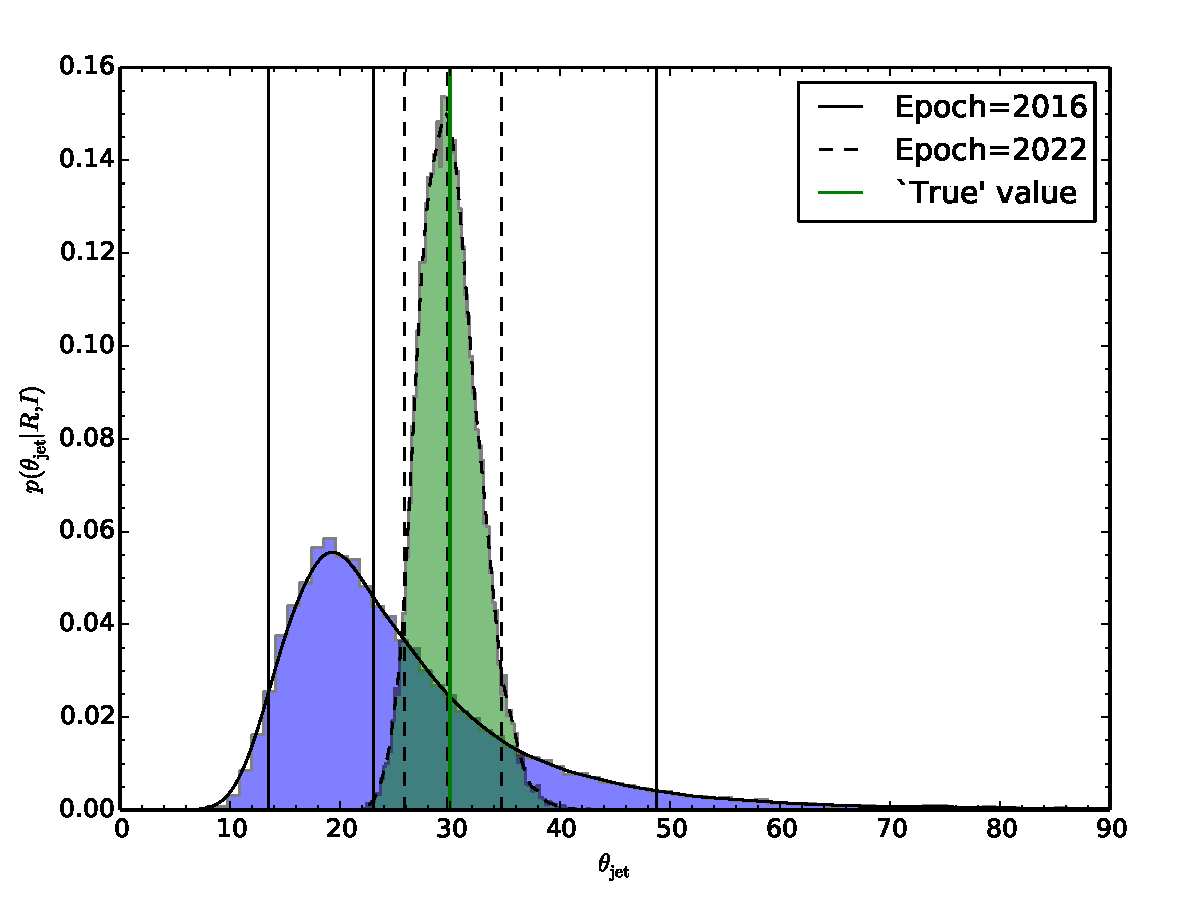
\includegraphics{example1.pdf}}
\end{figure}
\end{frame}

\begin{frame}
\frametitle{Example 2: unknown efficiency, uniform prior}
$\epsilon=0.5$, $p(\epsilon)=U(0,1)$, $\theta=30^{\circ}$\\~\\
Lines: 95\% confidence interval about median
\begin{figure}
    \centering
    \scalebox{0.4}{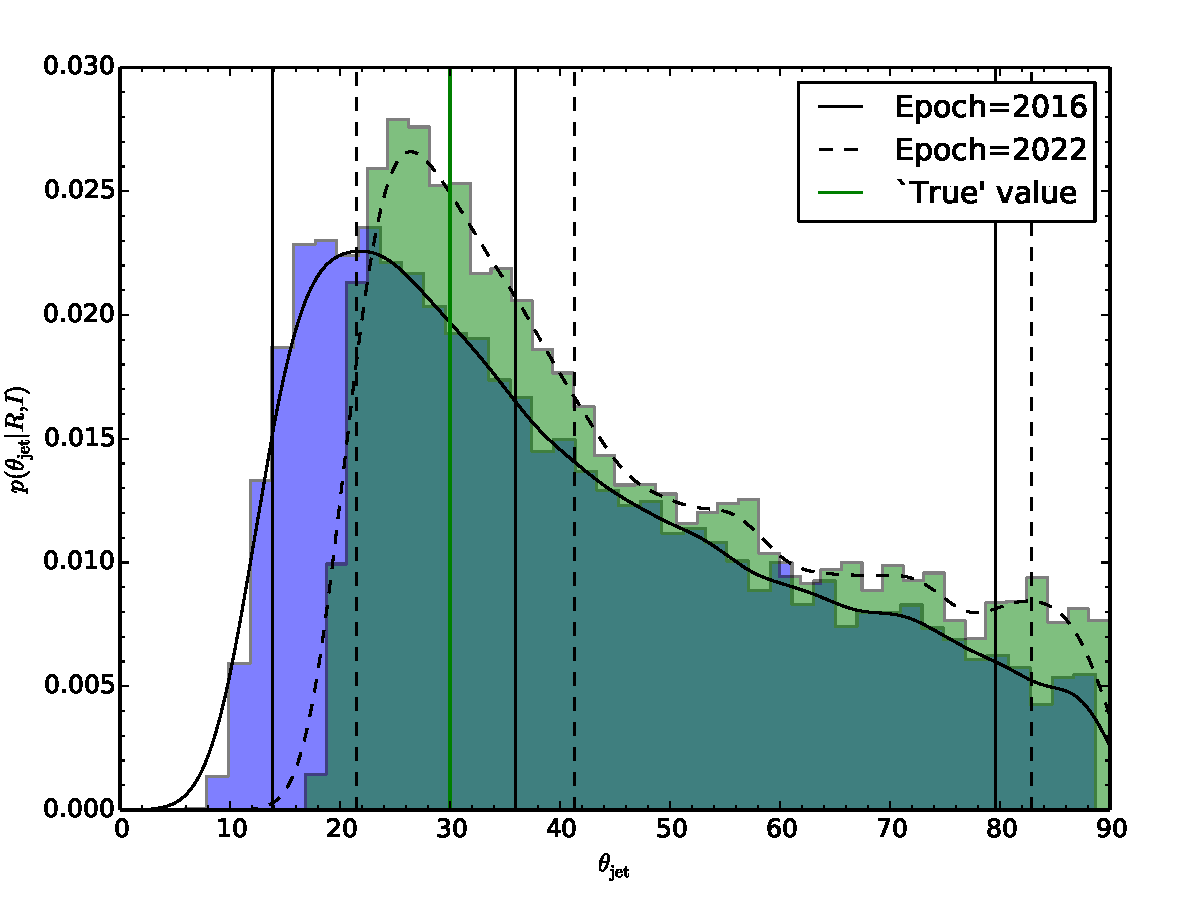
\includegraphics{example2.pdf}}
\end{figure}
\end{frame}

\begin{frame}
\frametitle{Example 3: unknown efficiency, Jeffreys prior}
$\epsilon=0.5$, $p(\epsilon)=\beta(0.5,0.5)$, $\theta=30^{\circ}$\\~\\
Lines: 95\% confidence interval about median
\begin{figure}
    \centering
    \scalebox{0.4}{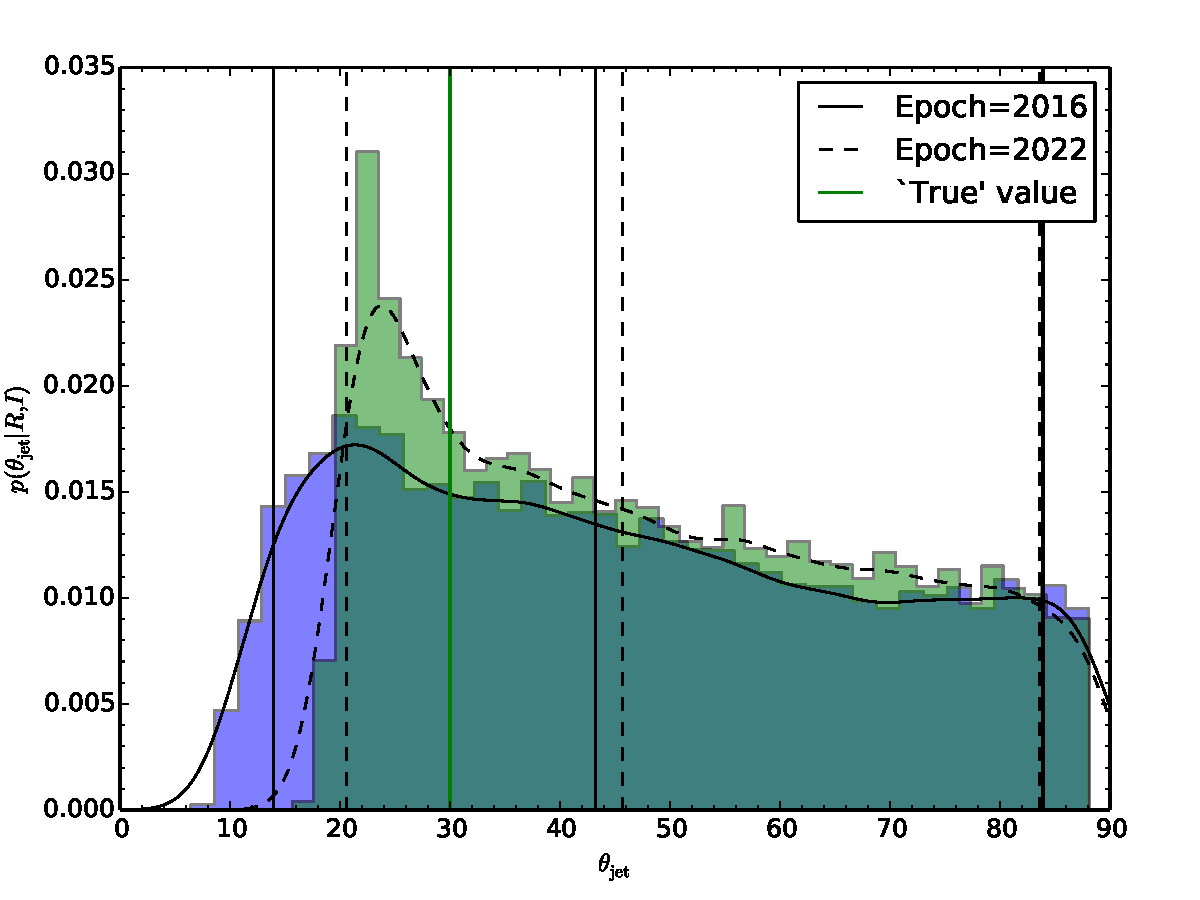
\includegraphics{example3.pdf}}
\end{figure}
\end{frame}

\end{document}
